\documentclass[12pt,a4paper]{article}
\usepackage[latin1]{inputenc}
\usepackage{float}
\usepackage{amsmath}
\usepackage{amsfonts}
\usepackage{amssymb}
\usepackage{graphicx}
\usepackage{fancyhdr}
\usepackage[hidelinks]{hyperref}

\pagestyle{fancy}
\fancyhf{}
\rfoot{Marco Gasperini - Ibrahim El Shemy - Davide Hu}
\title{\textbf{\Huge{HYPERMEDIA WEBSITE PROJECT}} \\ \large Design Document}
\author{Marco Gasperini - 10533178@polimi.it\\ Ibrahim El Shemy - 10491265@polimi.it \\ Davide Hu - 10493858@polimi.it}
\date{A.Y. 2018/2019 ??/??/???? delivery date}

\begin{document}
\maketitle
\newpage
\tableofcontents
\newpage

\section{Abstract}
During the implementation of a Web App the first step is making a document that describes the structure and shows the design model.\\For this purpose we have used the schemes C, L - IDM which show respectively:
\begin{itemize}
\item The conceptual model and the decisions related to it
\item The logical scheme in detail
\end{itemize}

\section{Design-in-the-large}
\subsection{C-IDM}
In this scheme we reported all the Topic, Kind of Topic, Group of Topic and Multiple Groups of Topic regarding the specifications, including the Relevant Relations and the requested cardinalities.
\begin{figure}[h]
\centering
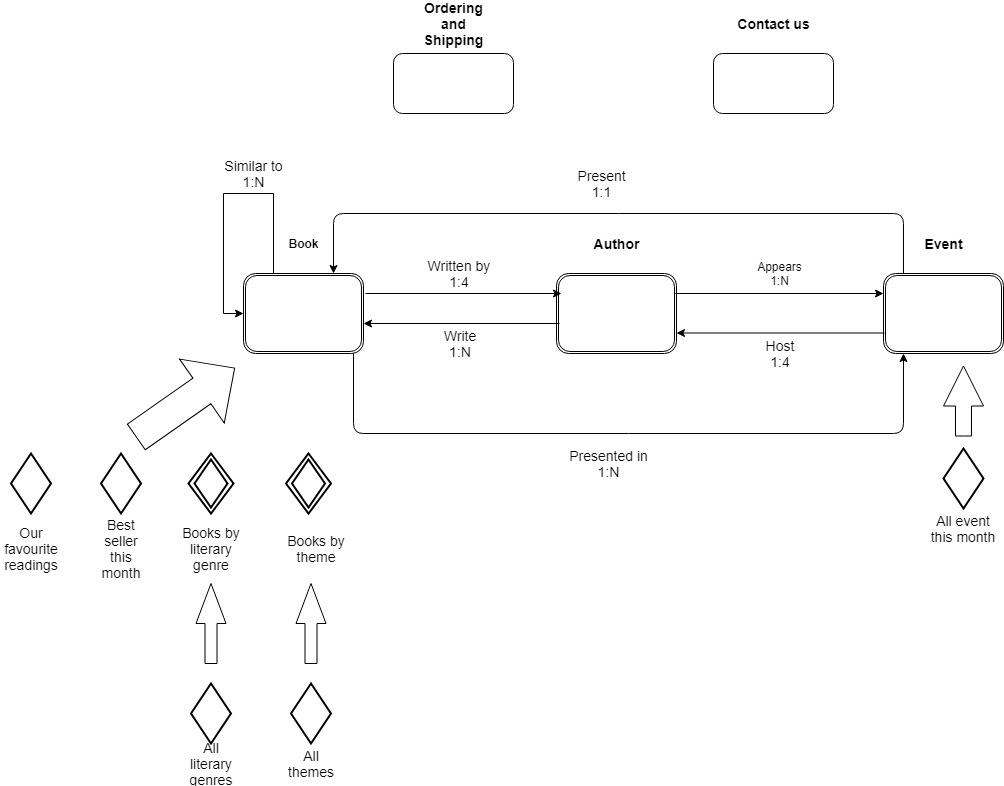
\includegraphics[width=0.9\linewidth]{imm.jpg}
\label{fig:IDM}
\end{figure}

\section{Design-in-the-small}
\subsection{L-IDM}
In the transaction from the conceptual scheme to the logical scheme, we added the Dialogue Acts concerning the Topics and Kind of Topics and the Introductory Dialogue Acts corresponding to the Group of Topic and the Multiple Groups of Topic, previously presented in the C-IDM.
\section{Design of DB}
\section{Scenarios}
In this section we can find three scenarios with a little description of them and some commented miniaturized screenshots that the user would traverse to execute the scenario.
\subsection{First scenario}
Elisabetta, is a big fan of the Harry Potter series. She would like to get in contact directly with the author of her favourite books, J. K. Rowling and so she decided to browse our website to find some events that may suite her desire. She visits the \textit{HomePage} and from there, she scroll down along the page and reads about the \textit{Event} page. She clicks on the \textit{Event} link and is redirected to a page where she can find a list of events. She finally finds an event that fulfills her needs and retreives information about the date and place. By clicking on the \textit{Show map} button she can also have an accurate information about where the event is held.\\\\
AGGIUNGERE SCREENSHOT DEI PASSAGGI!
\subsection{Second scenario}
Giovanni and Gianluca are two friends that share together the passion of reading and both are registered to our website. Since Gianluca's birthday is in a couple of day, Giovanni decides to gift him a book. From the \textit{HomePage} he clicks on the \textit{Book} landmark and is suddenly redirected to a page where he can find several books. He chooses one of them by clicking on it and the by clicking on the \textit{Add to cart} button he adds it to the shopping cart. He then visits the \textit{Shop} page where he complete the payment by clicking on the \textit{Process payment} button.\\\\
AGGIUNGERE SCREENSHOT DEI PASSAGGI!
\subsection{Third scenario}
Federico is a high school student and needs to do some homework research about an author of the Italian literature, Paolo Giordano. He visits our \textit{HomePage}, and by scrolling down he finds a link, \textit{Author}, with an image and some brief description about what he will find in that page. He clicks on the link and then is redirected to a page where he finds a list of different authors. He looks for Paolo Giordano, and by clicking on his image he can retrieve all the information he needed.\\\\
AGGIUNGERE SCREENSHOT DEI PASSAGGI!
\end{document}